% System Architecture Diagram for Biological Countercurvature Framework
% TikZ diagram showing the complete framework

\begin{figure}[h!]
\centering
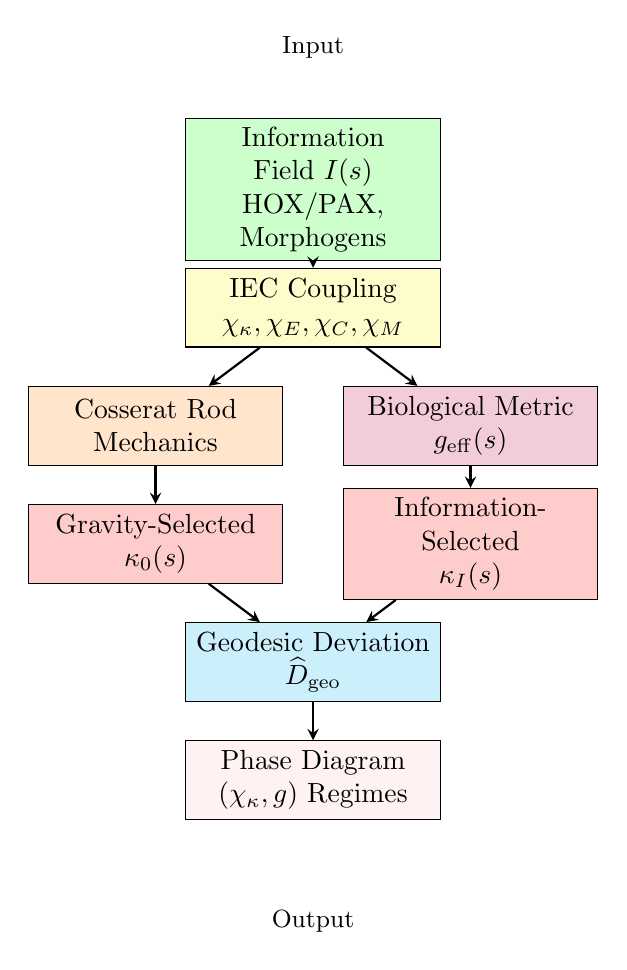
\begin{tikzpicture}[
    node distance=1.5cm,
    box/.style={rectangle, draw, fill=blue!10, text width=3cm, text centered, minimum height=1cm},
    arrow/.style={->, >=stealth, thick},
    label/.style={font=\small}
]

% Information Field Layer
\node[box, fill=green!20] (info) {Information Field $I(s)$\\HOX/PAX, Morphogens};

% IEC Coupling Layer
\node[box, fill=yellow!20, below of=info] (iec) {IEC Coupling\\$\chi_{\kappa}, \chi_{E}, \chi_{C}, \chi_{M}$};

% Cosserat Rod Layer
\node[box, fill=orange!20, below of=iec, xshift=-2cm] (cosserat) {Cosserat Rod\\Mechanics};

% Countercurvature Metric Layer
\node[box, fill=purple!20, below of=iec, xshift=2cm] (metric) {Biological Metric\\$g_{\mathrm{eff}}(s)$};

% Curvature Profiles
\node[box, fill=red!20, below of=cosserat] (kappa0) {Gravity-Selected\\$\kappa_{0}(s)$};

\node[box, fill=red!20, below of=metric] (kappaI) {Information-Selected\\$\kappa_{I}(s)$};

% Geodesic Deviation
\node[box, fill=cyan!20, below of=kappa0, xshift=2cm] (dgeo) {Geodesic Deviation\\$\widehat{D}_{\mathrm{geo}}$};

% Phase Diagram
\node[box, fill=pink!20, below of=dgeo] (phase) {Phase Diagram\\$(\chi_{\kappa}, g)$ Regimes};

% Arrows
\draw[arrow] (info) -- (iec);
\draw[arrow] (iec) -- (cosserat);
\draw[arrow] (iec) -- (metric);
\draw[arrow] (cosserat) -- (kappa0);
\draw[arrow] (metric) -- (kappaI);
\draw[arrow] (kappa0) -- (dgeo);
\draw[arrow] (kappaI) -- (dgeo);
\draw[arrow] (dgeo) -- (phase);

% Labels
\node[label, above of=info, yshift=0.3cm] {Input};
\node[label, below of=phase, yshift=-0.3cm] {Output};

\end{tikzpicture}
\caption{System architecture of the biological countercurvature framework. The information field $I(s)$ (top) drives IEC coupling parameters, which modify both Cosserat rod mechanics and the biological metric $g_{\mathrm{eff}}(s)$. The resulting curvature profiles $\kappa_{0}(s)$ and $\kappa_{I}(s)$ are compared via the geodesic deviation $\widehat{D}_{\mathrm{geo}}$, which maps to countercurvature regimes in the $(\chi_{\kappa}, g)$ phase diagram.}
\label{fig:system_architecture}
\end{figure}

